\chapter{Bell 202 on VHF}

The most common layer 1 modulation used for APRS on RF is a variant of the
Bell 202 audio frequency shift keyed (AFSK) modem transmitted via 
FM VHF radios. Each region has agreed on a local primary frequency for
APRS operations; 144.390MHz in Northern America, 144.800MHz in Europe, etc.

TODO The limited 1200 is important

\section{History of Bell 202}
\label{sec:bell202history}

\begin{figure}
	\centering
	\includegraphics[width=0.7\textwidth]{src/bell202sample}
	\caption{Typical Bell 202 baseband signal}
	\label{fig:bell202sample}
\end{figure}

Bell 202 is based on shifting between 1200Hz and 2200Hz tones to
represent a binary one or zero respectively as a rate of 
1200 symbols per second.
Originally developed by AT\&T for use on the telephone network \cite{202tspec},
it was selected for amateur radio packet operations due to the abundance
of modems available on the second-hand market in 1981 when the FCC authorized
amateur packet operations.

Due to Amateur radio operators
using Bell 202 as a physical layer below AX.25, which is a derivative of
X.25, it implicitly includes High-Level Data Link Control (HDLC) 
framing and bit stuffing in the layer 1 protocol \cite{n1vgphy}.
This means that the original 1200Hz mark and 2200Hz space symbols
do not directly represent one and zero.
The AX.25 data stream is encoded using the 
inverted non-return to zero (NRZI) encoding,
which requires zeros in the original bit stream to be encoded as a change
between 1200Hz and 2200Hz and ones to be encoded as transmitting the same
tone during two consecutive symbol periods \cite{iso13239}.

HDLC also requires that individual frames are delineated by the bit sequence
``0111 1110" (0x7E), which means that any string of five or more ones in the
frame's payload needs to be escaped using what's called ``bit stuffing"
to prevent the receiver from falsely detecting an end of frame early.
On the transmitting side, any sequence of five ones in the frame payload
has a zero appended to it, and on the receiving side a sequence of
five ones followed by a zero causes the receiver to 
drop the succeeding zero \cite[\S3.6]{ax25spec}.


\section{Bell 202 Transmission Format}

Despite being widely used for the majority of amateur packet radio operations, 
the combination of Bell 202 and HDLC as applied is not thoroughly documented 
as a stand-alone specification \cite{n1vgphy}\cite{aprsunveiled}.

\begin{figure}
	\centering
	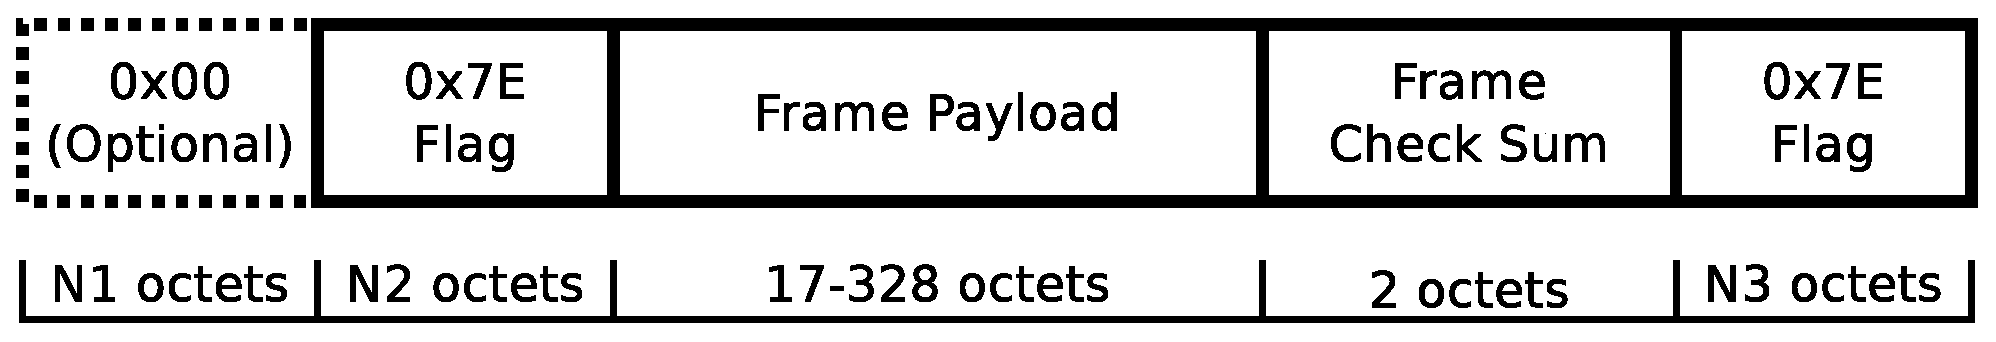
\includegraphics[width=1.0\textwidth]{src/dia/bell202}
	\caption{Bell 202/HDLC frame format}
	\label{fig:bell202format}
\end{figure}

Figure \ref{fig:bell202format} diagrams a typical single frame
Bell 202 transmission. There are a number of things to
consider:
\begin{itemize}
	\item The leading 0x00 octets are mentioned in very few documents
		discussing Bell 202, yet they significantly improve modem
		throughput \cite{millerinterview}. 
		0x00 encoded in NRZI causes a symbol transition
		every clock cycle and thus provides a more effective clock 
		syncronization target than the specified 0x7E octets. 0x7E is actually 
		the longest allowable string of 1s in the frame and 
		therefore has the lowest amount of energy at the clocking frequency
		and is remarkably the worst octet for modem syncronization.
	\item There is little guidance on the numer of flag octets before
		or after frames (represented by N2 and N3 in 
		figure \ref{fig:bell202format})
		beyond stating that there must be at least one. The sum of
		N1 and N2 is controllable in most modems via the ``TXDelay" parameter,
		which is discussed in section \ref{sec:kissparm}.
	\item It is permissible to encode multiple 
		frames per transmission, yet there is no guidance as to how
		many octets of 0x7E be included between them.
		Most modems insert several 0x7E octets between 
		frames.\footnote{For a specific example, the Argent Data OT3m TNC 
			with firmware r56474 inserts 3 flags before
		a frame, 7 flags between two frames, and 5 flags after the final frame.}
		Tests indicate that the number of flags between frames 
		significantly impacts throughput of the subsequent frame;
		quantitative measurements of this effect are beyond the 
		scope of this work.
	\item The frame payload and frame check sum must be bit stuffed as
		discussed in section \ref{sec:bell202history}
	\item Every octet is encoded and transmitted least significant bit first,
		including the Frame Check Sum.
		This contradicts the AX.25 and ITU V.42 specifications, 
		which state
		that while the frame payload is transmitted LSB first, the frame
		check sum is transmitted MSB first 
		\cite[\S3.8]{ax25spec},\cite{n1vgphy},\cite[\S8.1.2.2-3]{ituv42}.
	\item The Frame Check Sum is calculated using the CRC-16-CCITT checksum
		with the polynomial representation 0x1021. 
		Note that the two octets are sent little-endian, not
		big-endian as is specified in ITU V.42 \S8.1.2.3 and is the
		convention for IP-based protocols.

\end{itemize}

\section{Limitations on Modem Performance}

TODO No FEC is severe limitation

TODO Emphasis / deemphasis problem is unsolvable

TODO Define Basic 3002 phone channel as good benchmark

\section{Carrier Sense Multiple Access}
\label{sec:bell202csma}

Since amateur Bell 202 is a half duplex modulation traditionally using FM voice 
transceivers, one of the challenges to packet radio is avoiding multiple stations
transmitting on the same channel at once. Other derivatives of ALOHAnet, such as 
the original half duplex 10Mbps Ethernet, have the advantage that transmitters can
at least sense when a collision has taken place and use that information to abort
the transmission of the rest of the frame.

Throughout the history of APRS, there have been 
countless debates as to the implications
of different CSMA algorithms and primarily 
the need for one at all versus an entirely 
stocastic channel access method. The argument follows that the majority of 
channel contention is between multiple clients trying to reach a single digipeater
across what is called a split horizon, where each of the clients can hear and be heard
by the digipeater, but are entirely unaware of each other. In these types of instances,
even an optimal CSMA algorithm will never correctly cause one of the stations to hold 
off until the end of the other's transmission due to the required information being
entirely unavailable.

Besides the degenerate case of ignoring the current channel status completely when 
deciding to transmit a pending frame, there are two major algorithms used for CSMA
in APRS;
DWait and P-persistent.

DWait is a deterministic algorithm where each station is assigned a fixed
``quiet time" after the end of another tranmission before they will begin a locally
pending tranmission. This lends itself well to very carefully designed networks
where the relative priority of each station is known and a corresponding DWait time
is set for each station where a shorter DWait will always gain the channel over a longer
one. The requirement for the network to have an overarching design doesn't lend itself
well to the national APRS network, but could be applied effectively for localized 
portions of the APRS network and for ``insular" networks built for special events or
private groups of amateurs.

P-persistent is a stochastic algorithm with two variables: the slot time, and the
probability that a station should transmit at the beginning of a slot. The slot time
should be set to as short of a time interval as possible during which a station can
reliabily identify another station as transmitting 
before beginning its own transmission.
The P value should be tuned based on how likely another station is to transmit 
considering the number of other stations with 
pending traffic attempting to gain the channel.

For a discussion on typical values used in these algorithms, 
see section \ref{sec:kissparm}.

